% Copyright (c) 2023 Zachary Todd Edwards
% MIT License

% Must be compiled with lualatex and -shell-escape
% gnuplot required
\documentclass{beamer}
\setbeamersize{text margin left=0.125in,text margin right=0.125in}

\usepackage{fontspec}
\setmainfont{ubuntu}[
    Path        =   ../common/fonts/,
    Extension   =   .ttf,
    UprightFont =   *-R,
    BoldFont    =   *-B,
]
\setmonofont{ubuntumono}[
  Path          =   ../common/fonts/,
  Extension     =   .ttf,
  UprightFont   =   *-R,
  BoldFont      =   *-B,
]

% Copyright (c) 2023 Zachary Todd Edwards
% MIT License

\usepackage{pgfplots}
\pgfplotsset{compat=1.17}
\usepackage{adjustbox}
\usepackage{float}
\usepackage{caption}

\usepackage{xcolor}
\definecolor{codegray}{RGB}{128,128,128}
\definecolor{line_color}{RGB}{0,51,160}
\definecolor{mark_color}{RGB}{177,2,2}
\definecolor{avg_color}{RGB}{255, 163, 0}

\usepackage{listings}
\lstset{
  language=C++, % choose the language of the code
  basicstyle=\ttfamily\footnotesize,
  numberstyle=\tiny\color{codegray},
  numbers=left, % where to put the line-numbers
  numbersep=5pt,
}

%For getting the average of a parametric equation using gnuplot
\usepackage{shellesc}

\newcounter{PolynomialID}
\newcommand\getPolynomialID{polynomial\thePolynomialID}
\newcommand{\polynomial}[3][0.9\columnwidth]{
  \begin{figure}[H]
    \begin{center}
      \begin{adjustbox}{width = #1}
        \begin{tikzpicture}
          \begin{axis}[
              axis lines=center,
              xmin=-6, xmax=6,
              ymin=-6, ymax=6,
              xtick={-5,-4,...,5},
              ytick={-5,-4,...,5},
              domain = -6:6,
              restrict y to domain=-20:20,
              xtick distance=1,
              ytick distance=1,
              grid=major,
              grid style = {solid},
              yticklabels={,,},
              xticklabels={,,},]
            \addplot[id=\getPolynomialID,samples=100,line_color,style={thick},smooth] {#2};
          \end{axis}
        \end{tikzpicture}
      \end{adjustbox}
    \end{center}
    \caption*{#3}
  \end{figure}
  \stepcounter{PolynomialID}
}

\newcounter{MarkID}
\newcommand\getMarkID{mark\theMarkID}

\newcounter{WaveID}
\newcommand\getWaveID{wave\theWaveID}
\newlength{\wavewidth}
\newcommand{\waveform}[4][0.9\columnwidth]{% args: size, function(x), marks, caption
  \setlength{\wavewidth}{#1}
  \begin{figure}[H]
    \begin{center}
      \begin{tikzpicture}
        \begin{axis}[
            axis lines=center,
            tick pos = right,
            width = \wavewidth,
            height = 0.19\wavewidth,
            xmin=0, xmax=4,
            ymin=-2, ymax=2,
            xtick={1,2,3},
            ytick={-1,0,1},
            domain = 0:4,
            restrict y to domain=-4:4,
            xtick distance=1,
            ytick distance=1,
            grid=major,
            grid style = {solid},
            yticklabels={,,},
            xticklabels={,,},]
          \addplot[id=\getWaveID,samples=400,line_color,style={thick},smooth] function{#2};
          \ifnum#3>0
            \addplot[id=\getMarkID,samples=#3,mark_color,only marks, mark=*] function{#2};
            \stepcounter{MarkID}
          \fi
        \end{axis}
      \end{tikzpicture}
    \end{center}
    \caption*{#4}
  \end{figure}
  \stepcounter{WaveID}
}

\newcommand{\criticalFrequency}[2][0.9\columnwidth]{% args: size, caption
  \setlength{\wavewidth}{#1}
  \begin{figure}[H]
    \begin{center}
      \begin{tikzpicture}
        \begin{axis}[
            axis lines=center,
            tick pos = right,
            width = \wavewidth,
            height = 0.19\wavewidth,
            xmin=0, xmax=4,
            ymin=-2, ymax=2,
            xtick={1,2,3},
            ytick={-1,0,1},
            domain = 0:4,
            restrict y to domain=-4:4,
            xtick distance=1,
            ytick distance=1,
            grid=major,
            grid style = {solid},
            yticklabels={,,},
            xticklabels={,,},]
          \addplot[id=\getWaveID,samples=400,line_color,style={thick},smooth] function{cos(2*2*pi*x + 0.5) - sin(2*2*pi*x) * tan(0.5)};
          \stepcounter{WaveID}
          \addplot[id=\getWaveID,samples=400,mark_color,style={thick},smooth] function{cos(2*2*pi*x + 0.8) - sin(2*2*pi*x) * tan(0.8)};
          \stepcounter{WaveID}
          \addplot[id=\getWaveID,samples=400,avg_color,style={thick},smooth] function{cos(2*2*pi*x + 0.2) - sin(2*2*pi*x) * tan(0.2)};
          \stepcounter{WaveID}
          \addplot[only marks, black, mark=*] coordinates
            {(0.23,-1.1) (0.48,1.1)
              (0.73,-1.1) (0.98,1.1)
              (1.23,-1.1) (1.48,1.1)
              (1.73,-1.1) (1.98,1.1)
              (2.23,-1.1) (2.48,1.1)
              (2.73,-1.1) (2.98,1.1)
              (3.23,-1.1) (3.48,1.1)
              (3.73,-1.1) (3.98,1.1)};
        \end{axis}
      \end{tikzpicture}
    \end{center}
    \caption*{#2}
  \end{figure}
}

\newcounter{PhasorID}
\newcommand\getPhasorID{phasor\thePhasorID}
\newcommand\genPhasorTableFilename{\jobname.\getPhasorID.table}

\newcommand{\calcPhasorAverage}[1][\genPhasorTableFilename]{% arg: filename
  \ShellEscape{gnuplot -e "stats '#1' using 1; x_avg = STATS_mean; stats '#1' using 2; y_avg = STATS_mean; set print '#1.avg'; print x_avg, y_avg"}%
}

% args: size, equation(t), period, marks, caption
% mark being 0 turns off the average indicator, 1 only average indicator, > 1 marks & average
\newcommand{\phasor}[5][0.9\columnwidth]{
  \begin{figure}[H]
    \begin{center}
      \begin{adjustbox}{width = #1}
        \begin{tikzpicture}
          \begin{axis}[
              axis lines=center,
              xmin=-4, xmax=4,
              ymin=-4, ymax=4,
              xtick={-3,-2,...,3},
              ytick={-3,-2,...,3},
              xlabel={$\Re$},
              ylabel={$\Im$},
              xtick distance=1,
              ytick distance=1,
              grid=major,
              grid style = {solid},
              yticklabels={,,},
              xticklabels={,,},]
            \addplot gnuplot[parametric,id=\getPhasorID,domain=0:8,samples=1000,line_color,style={thick},smooth,solid, no markers] {
                (#2) * cos((-2 * pi * t) * (#3)),
                (#2) * sin((-2 * pi * t) * (#3))
              };
            \ifnum#4>1
              \addplot gnuplot[parametric,id=\getMarkID,domain=0:4,samples=#4,mark_color,only marks, mark=*] {
                  (#2) * cos((-2 * pi * t) * (#3)),
                  (#2) * sin((-2 * pi * t) * (#3))
                };
              \stepcounter{MarkID}
            \fi
            \ifnum#4>0
              \calcPhasorAverage
              \addplot[mark=*,avg_color] table {\genPhasorTableFilename.avg};
            \fi
          \end{axis}
        \end{tikzpicture}
      \end{adjustbox}
    \end{center}
    \caption*{#5}
  \end{figure}
  \stepcounter{PhasorID}
}

\newcommand{\unitCircle}[1][0.9\columnwidth]{
  \begin{figure}[H]
    \begin{center}
      \begin{adjustbox}{width = #1}
        \begin{tikzpicture}
          \begin{axis}[
              axis lines=center,
              axis equal,
              enlargelimits,
              xmin=-1, xmax=1,
              ymin=-1, ymax=1,
              xlabel={$\Re$},
              ylabel={$\Im$},
              ticks = none,
              thick]
            \draw[radius = 1] (0,0) circle;
            \draw[avg_color] (0,0) -- (0.125,0) arc[start angle=0, end angle=45,radius=0.125] node[avg_color, right]{\theta};
            \draw[black] (0,0) -- (45:1) node[black, midway, above left]{1} node[black,above right]{$e^{i\theta}$};
            \draw[mark_color] (0,0) -- (0.70710678118,0) node[mark_color, midway, below right]{$cos(\theta)$};
            \draw[line_color] (0.70710678118,0) -- (0.70710678118,0.70710678118) node[line_color, fill = white, midway, right]{$i \cdot sin(\theta)$};
            %this was genuinely the easiest way to draw a dot here
            \addplot[black,mark=*] coordinates {(0.70710678118,0.70710678118)};
          \end{axis}
        \end{tikzpicture}
      \end{adjustbox}
    \end{center}
    \caption*{The Complex Unit Circle}
  \end{figure}
}

\newcounter{SpectrumID}
\newcommand\getSpectrumID{spectrum\theSpectrumID}
\newcommand\genSpectrumTableFilename{\jobname.\getSpectrumID.table}

\newcommand{\genInitSpectrumTable}[4][\genSpectrumTableFilename]{% arg: filename, upper bound, samples, equation(x)
  \ShellEscape{gnuplot -e "set table '#1'; set samples #3; set dummy x; plot [x=0:#2] (#4);"}%
  \ShellEscape{perl ../common/fft.pl '#1' #2}%
}
% arg: size, seconds, window, samples, equation(x), caption
\newcommand{\fourierSpectrum}[6][0.9\columnwidth]{
  \begin{figure}[H]
    \begin{center}
      \begin{adjustbox}{width = #1}
        \begin{tikzpicture}
          \begin{axis}[
              axis lines = left,
              tick align = inside,
              xmin=0, xmax=#3,
              ymin=0, ymax=1,
              xtick distance = 1,
              ytick distance = 1,
              ytick={0.25,0.5,0.75},
              grid=major,
              grid style = {solid},
              xlabel = {Frequency Bin},
              ylabel = {Magnitude},
              x label style={at={(axis description cs:0.5,-0.1)},anchor=north},
              y label style={at={(axis description cs:-0.1,.5)},anchor=south},]
            \genInitSpectrumTable{#2}{#4}{#5}
            \ifnum#4>64
              \addplot[mark=none,line_color,smooth,thick,fill] table {\genSpectrumTableFilename};
            \else
              \addplot[only marks, mark=*,line_color] table {\genSpectrumTableFilename};
            \fi
          \end{axis}
        \end{tikzpicture}
      \end{adjustbox}
    \end{center}
    \caption*{#6}
  \end{figure}
  \stepcounter{SpectrumID}
}

\newcommand{\rootsOfUnity}[1][0.9\columnwidth]{
  \begin{figure}[H]
    \begin{center}
      \begin{adjustbox}{width = #1}
        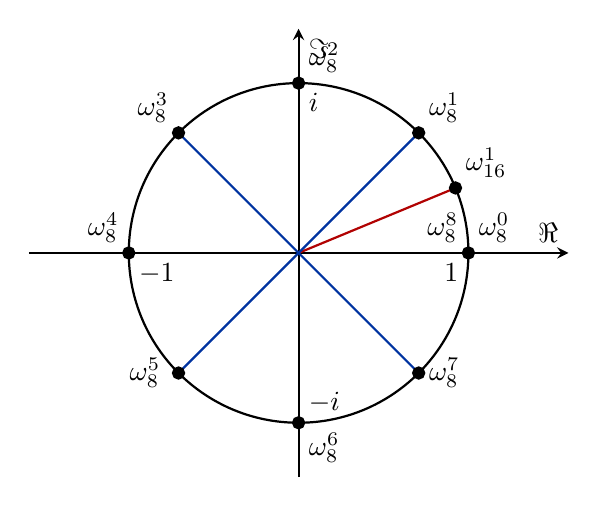
\begin{tikzpicture}
          \begin{axis}[
              axis lines=center,
              axis equal,
              enlargelimits,
              xmin=-1, xmax=1,
              ymin=-1.1, ymax=1.1,
              xlabel={$\Re$},
              ylabel={$\Im$},
              ticks = none,
              thick]
            \draw[radius = 1] (0,0) circle;
            \draw[mark_color] (0,0) -- (0.92387953251,0.38268343236);
            \addplot[black,mark=*] coordinates {(0.92387953251,0.38268343236)} node[above right] {$\omega_{16}^1$};
            \draw[line_color] (0,0) -- (0.70710678118,0.70710678118);
            \draw[line_color] (0,0) -- (-0.70710678118,0.70710678118);
            \draw[line_color] (0,0) -- (-0.70710678118,-0.70710678118);
            \draw[line_color] (0,0) -- (0.70710678118,-0.70710678118);
            \addplot[black,mark=*] coordinates {(1,0)} node[above right] {$\omega_8^0$} node[above left] {$\omega_8^8$} node[below left] {$1$};
            \addplot[black,mark=*] coordinates {(0.70710678118,0.70710678118)} node[above right] {$\omega_8^1$};
            \addplot[black,mark=*] coordinates {(0,1)} node[above right] {$\omega_8^2$} node[below right] {$i$};
            \addplot[black,mark=*] coordinates {(-0.70710678118,0.70710678118)} node[above left] {$\omega_8^3$};
            \addplot[black,mark=*] coordinates {(-1,0)} node[above left] {$\omega_8^4$} node[below right] {$-1$};
            \addplot[black,mark=*] coordinates {(-0.70710678118,-0.70710678118)} node[left,xshift=-0.1cm] {$\omega_8^5$};
            \addplot[black,mark=*] coordinates {(0,-1)} node[below right] {$\omega_8^6$} node[above right] {$-i$};
            \addplot[black,mark=*] coordinates {(0.70710678118,-0.70710678118)} node[right] {$\omega_8^7$};
          \end{axis}
        \end{tikzpicture}
      \end{adjustbox}
    \end{center}
    \caption*{The 8th Roots of Unity and First 16th Root of Unity}
  \end{figure}
}

\newcounter{ButterflyID}
\newcommand\getButterflyID{butterfly\theButterflyID}
\newcommand\genButterflyFilename{\jobname.\getButterflyID.out}

\newcommand{\genButterflyDIF}[2][\genButterflyFilename]{% arg: filename, samples
  \ShellEscape{perl ../common/butterfly-dif.pl #2 > '#1'}%
}

\usetikzlibrary {arrows.meta}

%args: size
\newcommand{\butterfly}[2][\linewidth]{
  \begin{figure}[H]
    \begin{center}
      \begin{tikzpicture}
        \begin{axis}[
            width = #1,
            axis line style={draw=none},
            tick style={draw=none},
            yticklabels={,,},
            xticklabels={,,},
          ] 
          \genButterflyDIF{#2}
          \input{\genButterflyFilename}
        \end{axis}
      \end{tikzpicture}
    \end{center}
    \caption*{The Cooley-Tukey Radix-2 Decimation-In-Frequency Fast Fourier Transform}
  \end{figure}
  \stepcounter{ButterflyID}
}
\captionsetup[figure]{font=small}

\usepackage{amsmath}

\title{The Fast Fourier Transform}
\author{Zachary Todd Edwards}
\date{\today}

\newcommand{\myWave}[1]{sin(2*2*pi*#1) + sin(3*2*pi*#1)}

\begin{document}
\frame{\titlepage}
\begin{frame}
  \frametitle{A Hard Problem}

  Lets say we have a wave that we want to find the component frequencies of:


  \waveform[\textwidth]{\myWave{x}}{0}{}

  We could try a brute force approach, look at the graphs of sums of sine waves until we get our original:

  \waveform[\textwidth]{sin(1*2*pi*x) + sin(1*2*pi*x)}{0}{1Hz + 1Hz}
  \waveform[\textwidth]{sin(1*2*pi*x) + sin(2*2*pi*x)}{0}{1Hz + 2Hz}
\end{frame}

\begin{frame}
  \waveform[\textwidth]{sin(1*2*pi*x) + sin(3*2*pi*x)}{0}{1Hz + 3Hz}
  \waveform[\textwidth]{sin(2*2*pi*x) + sin(2*2*pi*x)}{0}{2Hz + 2Hz}
  \waveform[\textwidth]{sin(2*2*pi*x) + sin(3*2*pi*x)}{0}{2Hz + 3Hz}
  \waveform[\textwidth]{sin(3*2*pi*x) + sin(3*2*pi*x)}{0}{3Hz + 3Hz}
\end{frame}
\begin{frame}
  Assumptions made:

  \begin{itemize}
    \item Amplitude centered at zero.
    \item Phase centered, not shifted left or right.
    \item All component frequencies were integer.
    \item Input was perfect, no noise.
  \end{itemize}

  Brute force was already not practical, these make it even worse!
\end{frame}
\begin{frame}

  Lets try visualizing it in a different way by wrapping our waveform around the origin of a graph:

  \begin{columns}
    \column{0.5\textwidth}
    \phasor{\myWave{t}}{1}{1}{Rotation Period = 1}
    \column{0.5\textwidth}
    \phasor{\myWave{t}}{2}{1}{Rotation Period = 2}
  \end{columns}
\end{frame}

\begin{frame}
  \begin{columns}
    \column{0.5\textwidth}
    \phasor{\myWave{t}}{3}{1}{Rotation Period = 3}
    \column{0.5\textwidth}
    \phasor{\myWave{t}}{4}{1}{Rotation Period = 4}
  \end{columns}

  The dot is the center or average of this wound up version of our waveform, and we can see that it is almost always very close to zero except when the rotation period is 3 or 2, which is also the component frequencies of our wave!

\end{frame}

\begin{frame}{Euler's Formula}
  How do we mathematically express this, is it actually any easier?

  \begin{itemize}
    \item Its not any simpler visually.
    \item Getting the average is an extra step.
    \item Rotation period seems vague and complicated.
  \end{itemize}


  The axis labels have already given away part of the secret, these wrappings are being graphed on the complex plane!
\end{frame}

\begin{frame}{Euler's Formula}
  \unitCircle[0.6\linewidth]
  \begin{center}
    $e^{i\theta}=cos(\theta)+i\cdot sin(\theta)$
  \end{center}
\end{frame}

\begin{frame}
  If $e^x$ is growth that is equal to its current value, and i is a right angle on the complex plane, $e^{ix}$ is rotation equal to its current value. This is a circle with a radius of 1. It is also worth noting that this is continuous and works for angles larger than $2\pi$ or less than 0.

\end{frame}

\begin{frame}{Spiralling a Function}

  Since Euler's formula always has a distance from the origin of 1 rotated by $\theta$ radians and multiplying anything by 1 is itself we can plug in our variable times $2\pi$ for $\theta$ and then multiply our function with that to wrap it around the origin!

  \begin{columns}
    \column{0.5\textwidth}
    \polynomial{x}{$F(x)=x$}
    \column{0.5\textwidth}
    \phasor{t}{1}{0}{$F(x)\cdot e^{ix2\pi}$ where $x \ge 0$}
  \end{columns}
\end{frame}

\begin{frame}
  The rotation period is how many full rotations we do for one unit increase to the input of our original function. We can adjust this is by multiplying $2\pi$ in the original formula. For a period of two we multiply it by two, etc. We can multiply by fractions to get periods under zero.

  \begin{columns}
    \column{0.5\textwidth}
    \phasor{t}{2}{0}{$F(x)\cdot e^{ix2\cdot 2\pi}$ where $x \ge 0$}
    \column{0.5\textwidth}
    \phasor{t}{3}{0}{$F(x)\cdot e^{ix3\cdot 2\pi}$ where $x \ge 0$}
  \end{columns}

\end{frame}

\begin{frame}
  \frametitle{The Continuous Fourier Transform}

  There is one last piece needed to get our winding solution to work: the average. Conveniently for us we have a quick way of getting the total area under a curve, we can take its integral and divide by the total time the wave occupies:

  \begin{displaymath}
    \hat{G}(f) = \frac{1}{N}\int_{0}^{N} G(x) \cdot e^{2\pi ifx}dx
  \end{displaymath}
\end{frame}

\begin{frame}
  This works! When graphed we will get something like this:

  \fourierSpectrum[0.7\linewidth]{4}{6}{512}{\myWave{x}}{$\hat{G}(f)$ for $G(x) = sin(2 \cdot 2\pi x) + sin(3 \cdot 2\pi x)$}
\end{frame}

\begin{frame}
  This is not quite the true Fourier transform though, there are a few adjustments to get there:

  \begin{itemize}
    \item No average, with the average it is sometimes called the ``normalized Fourier transform.''
    \item No time frame, runs from $-\infty$ to $+\infty$.
    \item Winding is done in clockwise direction, negative exponent.
    \item Variable being integrated is usually $t$.
  \end{itemize}

  With all this:

  \begin{displaymath}
    \hat{G}(f) = \int_{-\infty}^{\infty} G(t) \cdot e^{-2\pi ift}dt
  \end{displaymath}

  There is just one problem: computers tend to not like continuity or infinity.

\end{frame}

\begin{frame}
  \frametitle{The Discrete Fourier Transform}

  Lets try taking discrete points on the waveform and sum up their results when multiplied with $e^{i\theta}$ at regular intervals.

  \waveform[\linewidth]{\myWave{x}}{32}{32 samples across 4 seconds, for a sample rate of 8 per second.}

  \begin{columns}
    \column{0.4\textwidth}
    \phasor{\myWave{t}}{3}{32}{Rotation Period = 3}
    \column{0.4\textwidth}
    \phasor{\myWave{t}}{4}{32}{Rotation Period = 4}
  \end{columns}
\end{frame}

\begin{frame}
  The discrete version of the Fourier transform should be relatively easy to reverse engineer:
  \begin{displaymath}
    X_k = \sum_{n=0}^{N-1} x_n \cdot e^{-\frac{i2\pi}{N}kn}
  \end{displaymath}
  It is convention to use $x_n$ for the input set and $X_n$ for the output set, both of size $N$. We might also want to normalize the output:
  \begin{displaymath}
    X_k = \frac{1}{N} \sum_{n=0}^{N-1} x_n \cdot e^{-{\frac{i2\pi}{N}kn}}
  \end{displaymath}

\end{frame}

\begin{frame}
  With all that we get the following for our graph:
  \fourierSpectrum[0.5\linewidth]{4}{8}{32}{\myWave{x}}{}
  This doesn't look right, there are peaks at 2hz and 3hz but also 5hz and 6hz, and it looks symmetrical. What is going on?
\end{frame}

\begin{frame}{Nyquist-Shannon}
  Our graph of the discrete Fourier transform above is actually correct, but the oddness in its results hints at a deeper problem we are bumping up against: how do we know how many points are enough?

  \criticalFrequency[\linewidth]{}

  All of these waveforms have the same samples at the same sample rate, these samples also have many different waves that could fit them, there are actually infinitely many waveforms that could fit any set of discrete points! We need some constraints on the waveform coming in in order to do anything useful with the samples.
\end{frame}

\begin{frame}
  The symmetry of our spectrum graphs above actually give us a hint about it, here is one with double the sample rate:
  \fourierSpectrum[0.5\linewidth]{4}{16}{64}{\myWave{x}}{}
  \vspace{-10pt}
  The results got more accurate, as expected, but the center of symmetry doubled as well. This ``center of symmetry'' is called the Nyquist limit, and is the highest frequency that discrete samples can represent without a loss in fidelity, half of our sample rate, non-inclusive.
\end{frame}

\begin{frame}
  Interpreting the results:
  \begin{itemize}
    \item $k\frac{f_s}{N}$ is the frequency of each index where $k$ is the index of the result, $f_s$ is the sample rate per-second, and $N$ is the total number of samples.
    \item The magnitude, absolute value, of each entry is usually what is graphed.
    \item The imaginary part of each entry tells us that frequency's phase, how much it is shifted left or right.
  \end{itemize}
\end{frame}

\begin{frame}[fragile]{Complex Programming}

  Most programming languages include complex numbers as part of their standard library, or as part of a common third party library.\\~\\
  C does some macro magic to ``overload'' the operators for complex types, but cannot overload the functions so there is a separate set of math functions for them, as well as a few macros for assignment:
  \begin{lstlisting}
  #include <complex.h>
  void dft(double complex *x, double complex *X, int N){
    for(int i = 0; i < N; i++)
      X[i] = CMPLX(0.0, 0.0);

    for(int k = 0; k < N; k++)
      for(int n = 0; n < N; n++)
        X[k] += x[n] * cexp(-(((I * 2 * M_PI) / N) * k * n));
  }
\end{lstlisting}
\end{frame}

\begin{frame}[fragile]
  C++ is similar but uses templates:
  \begin{lstlisting}
  #include <complex>
  using namespace std;
  void dft(complex<double> *x, complex<double> *X, int N){
    for(int i = 0; i < N; i++)
      X[i] = {0.0, 0.0};

    for(int k = 0; k < N; k++)
      for(int n = 0; n < N; n++)
        X[k] += x[n] * exp(-(((1.0i * 2 * M_PI) / N) * k * n));
  }
\end{lstlisting}
\end{frame}
\begin{frame}[fragile]

  Perl:
  \begin{lstlisting}[language=Perl]
  use Math::Complex;
  sub DFT{
    my ($x, $X) = @_;
    my $N = scalar(@$x);
    @$X = ();

    for(my $k = 0; $k < $N; $k++){
      for(my $n = 0; $n < $N; $n++){
        $$X[$k] += $$x[$n] * exp(-(((i * 2 * pi) / $N)
                                 * $k * $n));
      }
    }
  }
\end{lstlisting}

  The complexity of this algorithm is $O(N^2)$, however, and we are going to want to be able to process frequencies in the gigahertz range. To make this practical we need to somehow speed this up.

\end{frame}
\begin{frame}[fragile]{A Simpler Problem}
  Lets tackle a similar but simpler problem, how can we get a set of points on a polynomial?

  Say we have a class for our points that looks like:
  \begin{lstlisting}
  class point{
    double x, y;
    point(_x, _y) : x(_x), y(_y){}
  };
\end{lstlisting}
  We might try to use the brute force method:
  \begin{lstlisting}
  vector<point> polynomial(int degree,
        double coefficients[], int n){
    vector<double> points(n);
    for(int x = 0; x < n; x++){
      double y = coefficients[0];
      for(int j = 1; j <= degree; j++)
        y += coefficients[j] * pow(x,j);
      points[x] = point(x,y);
    }
    return samples;
  }
\end{lstlisting}
\end{frame}

\begin{frame}
  This takes $O(nk)$ time where n is the degree of the polynomial and k is the number of samples needed. Is there a faster way?
\end{frame}

\begin{frame}
  \frametitle{Symmetry}
  Lets look at a few graphs of polynomials:

  \begin{columns}
    \column{0.5\textwidth}
    \polynomial{2*x}{$F(x)=2x$}
    \column{0.5\textwidth}
    \polynomial{1/2*x^2}{$F(x)=\frac{1}{2} x^2$}
  \end{columns}
\end{frame}

\begin{frame}
  \begin{columns}
    \column{0.5\textwidth}
    \polynomial{x^2+x^3}{$F(x)=x^2+x^3$}
    \column{0.5\textwidth}
    \polynomial{3*x^3-x^4}{$F(x)=3x^3-x^4$}
  \end{columns}
\end{frame}

\begin{frame}
  \begin{columns}
    \column{0.5\textwidth}
    \polynomial{x+(1/3)*x^3}{$F(x)=x+\frac{1}{3}x^3$}
    \column{0.5\textwidth}
    \polynomial{x^4+1}{$F(x)=x^4+1$}
  \end{columns}
\end{frame}

\begin{frame}
  Observations:
  \begin{itemize}
    \item Some are symmetrical across the vertical axis.
    \item Some are symmetrical across both axes.
    \item Some are not symmetrical across either axis.
  \end{itemize}

  The polynomials with only even-powered terms or odd-powered terms are symmetrical, with the former being across the vertical axis: $F(x) = F(-x)$, and the latter being symmetrical across both: $F(x) = -F(-x)$.\\~\\

  How can we take advantage of this?

\end{frame}

\begin{frame}{Polynomial Decomposition}
  Lets take the following rather wooly polynomial:
  \polynomial[0.6\textwidth]{x-3*x^2+2*x^3+4*x^4+x^5-1}{$F(x)=-1+x-3x^2+2x^3+4x^4+x^5$}
\end{frame}

\begin{frame}
  Lets try separating it into its odd and even terms:

  \begin{columns}
    \column{0.5\textwidth}
    \polynomial{-1-3*x^2+4*x^4}{$F_e(x)=-1-3x^2+4x^4$}
    \column{0.5\textwidth}
    \polynomial{x+2*x^3+x^5}{$F_o(x)=x+2x^3+x^5$}
  \end{columns}

  These are both symmetrical and when added together we get our original polynomial, we might be able to work with this.

\end{frame}

\begin{frame}[fragile]

  Lets try writing another algorithm to take advantage of this, to try to keep it as simple as possible we will assert that n, the number of points we want, is even:

  \begin{lstlisting}
  vector<point> points;
  assert(!(n % 2));
  for(int x = 1; x <= n / 2; x++){
    double yp = coefficients[0];
    double yn = coefficients[0];
    for(int j = 1; j <= degree; j++){
      double term = pow(x,j);
      yp += term;
      yn += (j % 2) ? -term : term;
    }
    points.push_back(point(x,yp));
    points.push_back(point(-x,yn));
  }
  return points;
\end{lstlisting}
\end{frame}

\begin{frame}
  Gross!
  \begin{itemize}
    \item Inelegant!
    \item Asymptotically the same.
  \end{itemize}

  We can factor an $x$ out of the odd terms so that we get $F_o(x)=x(1+2x^2+x^4)$ or $x F_o(x)=1+2x^2+x^4$. Putting this together we get $F(x) = F_e(x) + xF_o(x)$ and now that $F_o(x)$ is all even terms it would be the same for positive and negative inputs.\\~\\
  This could possibly eliminate the ternary operator above which might benefit performance a bit, but we are still stuck with the same complexity.

  To get any noticeable benefit we need a way to do this recursively.
\end{frame}

\begin{frame}
  We can start by trying to make $F_e(x)$ and $F_o(x)$ polynomials with their own odd and even terms. All of the terms in each of these are even, so we could divide the exponents by two and square the inputs. This gives us $F_e(x)=-1-3x+4x^2$ and $F_o(x)=1+2x+x^2$ resulting in our original polynomial being $F(x) = F_e(x^2) + x F_o(x^2)$.\\~\\

  This does not work recursively! Squaring the input makes it positive and changes its magnitude, this only works with inputs of 0 and 1 for real numbers.\\~\\

  We used the complex exponential $e^{ix}$ as a kind of ``1'' before, would it work here?
\end{frame}

\begin{frame}{The Roots of Unity}
  \rootsOfUnity[0.6\textwidth]
\end{frame}

\begin{frame}
  \begin{itemize}
    \item For real numbers $\sqrt{1}$ has two answers, 1 and -1, same for complex numbers.
    \item For real numbers $\sqrt[3]{1}$ has only one answer, 1, complex numbers have three answers: 1, $e^\frac{i2\pi}{3}$, $e^\frac{i4\pi}{3}$.
    \item Higher roots have more complex results; the n-th root of 1 has n complex values and these are the roots of unity.
    \item The first root of unity after 1 is generally denoted with $\omega$ (omega).
    \item The j-th root of unity for the n-th complex root of 1 would be $\omega_n^j$.
  \end{itemize}

\end{frame}

\begin{frame}
  Useful properties:
  \begin{itemize}
    \item Always add up to zero.
    \item Absolute value is always one.
    \item All equivalent ratios of $j$ and $n$ for $\omega_n^j$ are equivalent eg $\omega_8^2 = \omega_4^1$.
    \item Negation ``flips'' their position eg $-\omega_8^1 = \omega_8^5$.
    \item They are cyclical when raised to a power or multiplied eg ${\omega_8^3}^{10} = \omega_8^3 \cdot \omega_8^{10} = \omega_8^{30} = \omega_8^6$.
  \end{itemize}
  Since getting the square root of a complex number is relatively trivial these properties lets us quickly get power-of-two-first-roots of unity by repeatedly getting the square root (raising to the power of $\frac{1}{2}$) of $\omega$.\\~\\
  The roots of unity can also be calculated using $e^\frac{i2\pi j}{n}$, this is equivalent to the exponential used in the discrete transform.
\end{frame}

\begin{frame}
  Complex numbers can be written as $a + bi$, with this the formula for getting the square root of a complex number is:
  \begin{displaymath}
    \sqrt{a+ib} = \pm\left(\sqrt{\frac{|z| + a}{2}} + i\sqrt{\frac{|z| - a}{2}}\right) \text{ when } b \ge 0
  \end{displaymath}
  \begin{displaymath}
    \sqrt{a+ib} = \pm\left(\sqrt{\frac{|z| + a}{2}} - i\sqrt{\frac{|z| - a}{2}}\right) \text{ when } b < 0
  \end{displaymath}

  The absolute value of a complex number is $\sqrt{a^2+b^2}$ and squaring a complex number is the same as real algebra, replacing $i^2$ with -1. If we are only dealing with $a + bi$ we can treat it like a binomial and the squaring formula is $a^2 - b^2 + 2abi$.
\end{frame}

\begin{frame}
  Lets run through a few examples to see all of this in action:
  \begin{columns}
    \column{0.5\textwidth}
    \begin{align*}
      \sqrt{1} & = \sqrt{\frac{|1| + 1}{2}} + i\sqrt{\frac{|1| - 1}{2}} \\
               & = \sqrt{\frac{2}{2}} + i\sqrt{\frac{2}{2}}             \\
               & = \sqrt{1} + i\sqrt{0}                                 \\
               & = -1 + 0i
    \end{align*}
    \column{0.5\textwidth}
    \begin{align*}
      (-1 + 0i)^2 & = (-1)^2 - (0)^2  \\
                  & \quad + 2(-1)(0)i \\
                  & = 1 - 0 + 0i      \\
                  & = 1               \\
    \end{align*}
  \end{columns}
\end{frame}

\begin{frame}
  \begin{columns}
    \column{0.6\textwidth}
    \begin{align*}
      \sqrt{-1} & = \sqrt{\frac{|-1| + -1}{2}} + i\sqrt{\frac{|-1| - -1}{2}} \\
                & = \sqrt{\frac{0}{2}} + i\sqrt{\frac{2}{2}}                 \\
                & = \sqrt{0} + i\sqrt{1}                                     \\
                & = 0 + 1i = i
    \end{align*}
    \column{0.4\textwidth}
    \begin{align*}
      i^2 = (0 + 1i)^2 & = (0)^2 - (1)^2  \\
                       & \quad + 2(0)(1)i \\
                       & = 0 - 1 + 0i     \\
                       & = -1
    \end{align*}
  \end{columns}
\end{frame}

\begin{frame}
  \begin{columns}
    \column{0.5\textwidth}
    \begin{align*}
      \sqrt{i} = \sqrt{0+1i} & = \sqrt{\frac{|0+1i| + 0}{2}}              \\
                             & \quad + i\sqrt{\frac{|0+1i| - 0}{2}}       \\
                             & = \sqrt{\frac{1}{2}} + i\sqrt{\frac{1}{2}} \\
                             & = \frac{1}{\sqrt{2}} + \frac{i}{\sqrt{2}}  \\
                             & = \frac{1+i}{\sqrt{2}}
    \end{align*}
    \column{0.5\textwidth}
    \begin{align*}
      \left(\frac{1+i}{\sqrt{2}}\right)^2 & = \frac{1+i}{\sqrt{2}} \cdot \frac{1+i}{\sqrt{2}} \\
                                          & = \frac{(1+i)(1+i)}{\sqrt{2}\cdot\sqrt{2}}        \\
                                          & = \frac{1+2i+i^2}{2}                              \\
                                          & = \frac{1+2i-1}{2}                                \\
                                          & = \frac{2i}{2}                                    \\
                                          & = i
    \end{align*}
  \end{columns}
\end{frame}

\begin{frame}{The Fast Fourier Transform}
  Putting all of this together:
  \begin{center}
    \begin{tabular}{llll}
      $F(x)$      & \multicolumn{2}{l}{$= -1+x-3x^2+2x^3+4x^4+x^5$} & $=F_e(x^2)+xF_o(x^2)$                                \\
      $F_e(x)$    & $=-1-3x+4x^2$                                   &                       & $=F_{ee}(x^2)+xF_{eo}(x^2)$  \\
      $F_o(x)$    & $=1+2x+x^2$                                     &                       & $= F_{oe}(x^2)+xF_{oo}(x^2)$ \\
      $F_{ee}(x)$ & $=-1+4x$                                        & $F_{eo}(x)=-3$        &                              \\
      $F_{oe}(x)$ & $=1+x$                                          & $F_{oo}(x)=2$         &                              \\
    \end{tabular}
  \end{center}
\end{frame}

\begin{frame}
  Plugging in our roots of unity:
  \begin{center}
    \begin{tabular}{ll | ll | ll}
      $F_{ee}(1)$  & $= 3$  & $F_e(1)$  & $= 0$       & $F(1)$         & $= 4$                    \\
      $F_{ee}(-1)$ & $= -5$ & $F_e(i)$  & $= 5 - 3i$  & $F(\omega)$    & $= - 5 - 3i + 2\omega i$ \\
      $F_{eo}(1)$  & $= -3$ & $F_e(-1)$ & $= 6$       & $F(i)$         & $= 6$                    \\
      $F_{eo}(-1)$ & $= -3$ & $F_e(-i)$ & $= -5 + 3i$ & $F(\omega i)$  & $= - 5 + 3i + 2\omega$   \\
      $F_{oe}(1)$  & $= 1$  & $F_o(1)$  & $= 2 + 2$   & $F(-1)$        & $= -4$                   \\
      $F_{oe}(-1)$ & $= 0$  & $F_o(i)$  & $= 2i$      & $F(-\omega)$   & $= - 5 - 3i - 2\omega i$ \\
      $F_{oo}(1)$  & $= 2$  & $F_o(-1)$ & $= 0$       & $F(-i)$        & $= 6$                    \\
      $F_{oo}(-1)$ & $= 2$  & $F_o(-i)$ & $= -2i$     & $F(-\omega i)$ & $= - 5 + 3i - 2\omega$   \\
    \end{tabular}
  \end{center}
\end{frame}

\begin{frame}
  Comparing the results with that of the discrete Fourier transform on the coefficients, padding with zeros to get the same number of outputs:\\~\\
  \begin{adjustbox}{width = \textwidth}
    \begin{tabular}{ |c|c|c|c|c|c|c|c|c| }
      \hline
      Input  & -1 & 1           & -3 & 2           & 4  & 1           & 0 & 0           \\
      \hline
      Output & 4  & -6.41-1.59i & 6  & -3.59+4.41i & -4 & -3.59-4.41i & 6 & -6.41+1.59i \\
      \hline
    \end{tabular}
  \end{adjustbox}\\~\\
  It is a perfect match, and with $O(NlogN)$ complexity!
\end{frame}

\begin{frame}[fragile]
  Lets write some code to calculate this, since the FFT can be calculated in-place X will be used as the input and overwritten:
  \begin{lstlisting}
  #include <complex>
  void fft(std::complex<double> *X, int N){
    std::complex<double> omega = -1;
    for (int n = 2; n <= N; n *= 2){
      for (int k = 0; k < N; k += n){
        for (int j = 0; j < n / 2; j++) {
          std::complex<double> product = 
            std::pow(omega,j) * X[k + j + n / 2];
          X[k + j + n / 2] = X[k + j] - product;
          X[k + j] = X[k + j] + product;
        }
      }
      omega = std::sqrt(omega);
    }
  }
\end{lstlisting}
\end{frame}

\begin{frame}
  Lets run it and see what it does:\\~\\
  \begin{adjustbox}{width=\textwidth}
    \begin{tabular}{ |c|c|c|c|c|c|c|c|c| }
      \hline
      Input  & -1 & 1        & -3       & 2         & 4  & 1         & 0        & 0        \\
      \hline
      Output & 4  & 0.1-2.9i & 1.0+5.0i & -4.1+7.1i & -6 & -4.1-7.1i & 1.0-5.0i & 0.1+2.9i \\
      \hline
    \end{tabular}
  \end{adjustbox}\\~\\
  This is not correct! This code is actually good, there is just one more thing we are missing.

\end{frame}

\begin{frame}{The Cooley-Tukey Radix-2 Decimation-In-Frequency Fast Fourier Transform}
  \begin{adjustbox}{width=\textwidth}
    \begin{tikzpicture}
      \begin{axis}[
          width = 1.4\textwidth,
          height = \textheight,
          axis line style={draw=none},
          tick style={draw=none},
          yticklabels={,,},
          xticklabels={,,},
        ]
        \genButterflyDIF{8}
        \input{\genButterflyFilename}
      \end{axis}
    \end{tikzpicture}
  \end{adjustbox}
  \stepcounter{ButterflyID}
\end{frame}

\begin{frame}
  Drawing out how values are reused we get something like the above, usually called a butterfly diagram. The part we are missing is the input ordering, we need to get the inputs in their order after the recursive even/odd separating.\\~\\
  This ordering is actually a little insidious, take a second to see if you can figure out a non-recursive way to describe the ordering.
\end{frame}

\begin{frame}
  The ordering is called bit-reversal-permutation, the index of each element in this ordering is the bits of the original index reversed. With the input in this order we, at last, get:\\~\\
  \begin{adjustbox}{width = \textwidth}
    \begin{tabular}{ |c|c|c|c|c|c|c|c|c| }
      \hline
      Input  & -1 & 1           & -3 & 2           & 4  & 1           & 0 & 0           \\
      \hline
      Output & 4  & -6.41-1.59i & 6  & -3.59+4.41i & -4 & -3.59-4.41i & 6 & -6.41+1.59i \\
      \hline
    \end{tabular}
  \end{adjustbox}
\end{frame}
\end{document}